\FILENAME

\chapter{Bare Metal}\label{bare-metal-user-guide}

In this page you will find documentation guiding you through the
bare-metal deployment features available in~Chameleon. Chameleon gives
users administrative access to bare-metal compute resources to
run~{cloud computing~}experiments with a high degree of customization
and repeatability. Typically, an experiment will go through several
phases, as illustrated in the figure below:

{
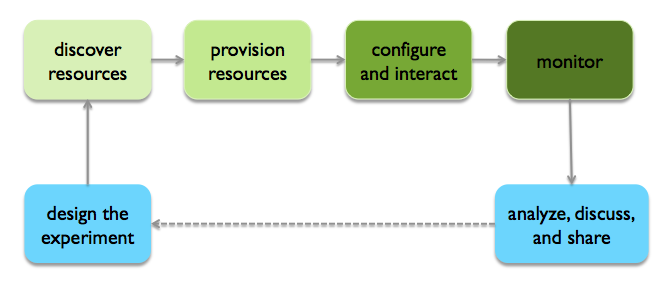
\includegraphics[width=\columnwidth]{images/chameleon/baremetal.png}
}

The bare-metal user guide comes in two editions. The first is how to use
Chameleon resources~via the web interface, the recommended choice for
new users to quickly learn how to use our testbed:

\textbf{\href{https://www.chameleoncloud.org/discover-resources}{Get
started with Chamelon using the web interface}}

\begin{enumerate}
\tightlist
\item
  \href{https://www.chameleoncloud.org/discover-resources/}{Discover
  Resources}
\item
  \href{https://www.chameleoncloud.org/provision-resources/}{Provision
  Resources}~
\item
  \href{https://www.chameleoncloud.org/configure-and-interact/}{Configure
  and Interact}
\item
  \href{https://www.chameleoncloud.org/monitor-and-collect/}{Monitor and
  Collect Results}
\end{enumerate}

The second targets~advanced users who are already familiar with
Chameleon~and would like to learn how to use Chameleon from the~command
line or with scripts.

\href{https://www.chameleoncloud.org/discover-resources-command-lines}{Get
started with Chameleon using the command line~(advanced)}

\begin{enumerate}
\tightlist
\item
  \href{https://www.chameleoncloud.org/discover-resources-command-lines/}{Discover
  Resources}
\item
  \href{https://www.chameleoncloud.org/advanced-provision-resources/}{Provision
  Resources}
\item
  \href{https://www.chameleoncloud.org/advanced-configure-and-interact/}{Configure
  and Interact}
\item
  \href{https://www.chameleoncloud.org/monitor-and-collect/}{Monitor and
  Collect Results}
\end{enumerate}

You do not need to strictly follow the documentation~sequentially.
However, note that some steps assume that~previous ones have been
successfully performed.

You can also consult~documentation~describing how to use advanced
features of Chameleon not covered by the guides above:

\begin{itemize}
\tightlist
\item
  the
  \href{https://www.chameleoncloud.org/docs/bare-metal-user-guide/chameleon-object-store/}{Chameleon
  Object Store},
\item
  \href{https://www.chameleoncloud.org/docs/bare-metal-user-guide/network-isolation-bare-metal/}{network
  isolation for bare metal}.
\end{itemize}


